\subsection{\texorpdfstring{\(C^{r,s}\) 类函数}{C\^{}\{r,s\} 类函数}}

在本条中，E 表示一个实 Banach 空间，F₁ 与 F₂ 是 K 上的 Banach 空间，V 是 E × F₁ 的开子集，f 是从 V 到 F₂ 的映射。给 E、F₁ 与 F₂ 装备与其 Banach 空间结构相容的范数。

15.1.1（“可微情形”）。假设 K = R 且 \(s \neq \omega\)。我们称 f 是 \(C_{R}^{r,s}\) 类（或简称 \(C^{r,s}\) 类）的，如果它具有迭代偏导数 \(D_{E}^{p}D_{F_{1}}^{q}f\)（1.7.2），且对每对正整数 \((p,q)\)（满足 \(p \leqslant r\) 与 \(p + q \leqslant s\)）都连续。等价地，迭代偏导数 \(D_{F_{1}}^{q}f\) 存在且都是 \(C^{r}\) 类的（对每个满足 \(0 \leqslant q \leqslant s - r\) 的整数 q）。若 s = r，这等价于说 f 是 \(C^{r}\) 类的；若 \(s \geqslant r + 1\)，这等价于说 f 是 \(C^{r}\) 类的且 \(D_{F_{1}}f\) 是 \(C^{r,s-1}\) 类的。

若 f 是 \(C^{r,s}\) 类的，且 \(p \leqslant r, p + q + 1 \leqslant s\)，则函数 \(D_{E}^{p}D_{F_{1}}^{q}f\) 有关于 \(F_{1}\) 的偏导数，由下式给出：

\[
\mathbf {D} _ {\mathbf {F} _ {1}} (\mathbf {D} _ {\mathbf {E}} ^ {p} \mathbf {D} _ {\mathbf {F} _ {1}} ^ {q} f) = \mathbf {D} _ {\mathbf {E}} ^ {p} \mathbf {D} _ {\mathbf {F} _ {1}} ^ {q + 1} f.\tag{1}
\]

15.1.2（“解析情形”）。我们假设 \(s = \omega\)。对每个整数 \(k \geqslant 0\)，用 \(\mathbf{P}_{k}(\mathbf{F}_{1}; \mathbf{F}_{2})\) 表示 \(k\) 次连续齐次多项式（\(\mathbf{F}_{1}\) 上、取值于 \(\mathbf{F}_{2}\) 的）全体组成的空间，装备第一分册附录 p. 88, A.2 中定义的范数。

我们称 \(f\) 是 \(\mathbf{C}_{\mathbf{K}}^{r,\omega}\) 类的（若对 K 没有歧义，也简称 \(\mathbf{C}^{r,\omega}\) 类），如果对每个点 \((x_{0},y_{0})\in\mathbf{V}\)，存在 \(x_{0}\) 在 E 中的邻域 U、实数 \textgreater 与 \(\geqslant\)，以及函数 \(h_{k}\colon\mathbf{U}\to\mathbf{P}_{k}(\mathbf{F}_{1};\mathbf{F}_{2})\)（\(k\in\mathbf{N}\)），它们是 \(\mathbf{C}^{r}\) 类的（对 K-流形 \(\mathrm{P}_{k}(\mathrm{F}_{1};\mathrm{F}_{2})\) 的结构之下的微分流形结构而言），使得：

\begin{enumerate}
\def\labelenumi{(\roman{enumi})}
\item
  \(\mathbf{U} \times (y_0 + \mathbf{B}(\mathbf{R})) \subset \mathbf{V}\)，其中 \(\mathbf{B}(\mathbf{R})\) 是半径为 \(\mathbf{R}\) 的开球（\(\mathbf{F}_1\) 中的）；
\item
  若 \(x \in \mathbf{U}\) 且 \(p \leqslant r\)，则有 \(\sum_{k=0}^{\infty} \| D^p h_k(x) \| R^k \leqslant M\)；
\item
  若 \(\mathrm{si} x \in \mathrm{U}\) 且 \(t \in \mathrm{B}(\mathbb{R})\)，则有 \(\sum_{k=0}^{\infty} h_k(x)(t) = f(x, y_0 + t)\)。
\end{enumerate}

这些性质蕴含：

\begin{enumerate}
\def\labelenumi{(\roman{enumi})}
\setcounter{enumi}{3}
\tightlist
\item
  对每个 \(t \in \mathbf{B}(\mathbf{R})\)，函数 \(x \mapsto f(x, y_0 + t)\) 在 U 中是 \(\mathbf{C}^{r}\) 类的，且有
\end{enumerate}

\[
\mathbf {D} _ {\mathbb {E}} ^ {p} f (x, y _ {0} + t) = \sum_ {k = 0} ^ {\infty} \mathbf {D} ^ {p} h _ {k} (x) (t) \quad \text { if } p \leqslant r \text { and } x \in \mathrm{U}.\tag{2}
\]

如果把上面的条件 (ii) 换成下面两个条件之一，\(C^{r,\omega}\) 类函数的定义不变：

(ii') 诸 \(h_k\) 定义一个 \(C^r\) 类态射，它从 U 映到 K-Banach 空间 \(\mathcal{H}_{\mathbb{R}}(\mathrm{F}_1; \mathrm{F}_2)\) 的底实 Banach 空间中（3.1.1 与 3.1.2）。

(ii'') 诸 \(h_k\) 定义一个 \(C'\) 类态射，它从 U 映到 K-Banach 空间 \(\tilde{\mathcal{H}}_R(F_1; F_2)\) 的底实 Banach 空间中（3.1.5）。

15.1.3. 假设 K = R。要使 f 是 \(C_{R}^{r,\omega}\) 类的，必须且只需 f 是 \(C^{r,\infty}\) 类的（15.1.1），且对每个 \((x_{0}, y_{0}) \in V\)，存在一个邻域 \(V_{0}\)（\((x_{0}, y_{0})\) 在 V 中的邻域）及正实数 A 与 M，使得

\[
\frac {1}{q !} \left\| \mathrm{D} _ {\mathbf {E}} ^ {p} \mathrm{D} _ {\mathbf {F} _ {1}} ^ {q} f (x, y) \right\| \leqslant \mathrm{A}. \mathrm{M} ^ {q}\tag{3}
\]

对所有 \(p \leqslant r\)、每个 \(q \geqslant 0\) 及每个 \((x, y) \in V_0\) 成立。

15.1.4. 假设 K = C。要使 f 是 \(C_{C}^{r,\omega}\) 类的，必须且只需下列两个条件满足：

\begin{enumerate}
\def\labelenumi{\alph{enumi})}
\item
  f 是 \(C_{R}^{r,\omega}\) 类的（对于 \(F_{1}\) 与 \(F_{2}\) 的底实结构）。
\item
  对每个 \((x, y) \in \mathbf{V}\)，\(\mathbf{D}_{\mathbb{F}_1} f(x, y)\) 是 \(\mathbf{C}\)-线性映射（从 \(\mathbf{F}_1\) 到 \(\mathbf{F}_2\)）。
\end{enumerate}

当 \(F_{1}\) 是有限维时，可以把 a) 换成：

\(\mathit{a}^{\prime})\) \(f\) 是 \(C^{r}\) 类的。

15.1.5. \(\mathbf{C}^{r,s}\) 类映射（从 V 到 \(\mathbf{F}_2\) 的映射）全体组成的集合与 E、\(\mathbf{F}_1\)、\(\mathbf{F}_2\) 上范数的选取无关。

15.1.6. 设 B 是一个 \(C^{r}\) 类微分流形，W 是 \(B \times F_{1}\) 的开子集，\(\rho\) 是从 W 到 \(F_{2}\) 的映射。设 \(c = (\mathrm{U}, \varphi, \mathrm{E}_{c})\) 是流形 B 的一个卡。用 \(W_{c}\) 表示 \(E_{c} \times F_{1}\) 中开子集，即在 \(\varphi \times Id_{F_{1}}\) 的作用下 \(W \cap (\mathrm{U} \times F_{1})\) 的像，并用 \(\rho_{c}\) 表示从 \(W_{c}\) 到 \(F_{2}\) 的满足下式的映射

\[
\rho_{c}(\varphi(x),y) = \rho(x,y) \quad \text { if } \quad (x,y) \in \mathbf{W} \cap (\mathbf{U} \times \mathbf{F}_{1}).
\]

称映射 \(\rho\colon\mathbf{W}\to\mathbf{F}_{2}\) 是 \(\mathbf{C}^{r,s}\) 类的，如果对流形 B 的每个卡 \(c\)，映射 \(\rho_{c}\colon\mathbf{W}_{c}\to\mathbf{F}_{2}\) 都是 15.1.1 与 15.1.2 意义下的 \(\mathbf{C}^{r,s}\) 类映射；只需对一个其定义域覆盖 B 的卡族验证该条件即可。这样的映射 \(\rho\) 是 \(\mathbf{C}^{r}\) 类的（对 \(\mathbf{B}\times\mathbf{F}_{1}\) 与 \(\mathbf{F}_{2}\) 的底实结构而言）；它限制在集合 \(\mathbf{W}\cap(\{b\}\times\mathbf{F}_{1})\) 上是一个 \(\mathbf{C}^{s}\) 类的 K-态射（对每个 \(b\in\mathbf{B}\)）。

15.1.7. 设 \(\mathbf{B}_1\) 与 \(\mathbf{B}_2\) 是 \(\mathbf{C}^r\) 类微分流形，并设 \(g: \mathbf{B}_1 \to \mathbf{B}_2\) 是一个

\pandocbounded{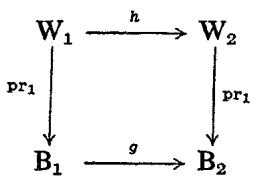
\includegraphics[keepaspectratio]{images/part001_9c3df15b.jpg}}

\(\mathbf{C}^{r}\) 类态射。设 \(\mathbf{W}_{1}\)（相应地，\(\mathbf{W}_{2}\)）是 \(\mathbf{B}_{1}\times\mathbf{F}_{1}\)（相应地，\(\mathbf{B}_{2}\times\mathbf{F}_{2}\)）的开子集，并设 \(h:\mathbf{W}_{1}\to\mathbf{W}_{2}\) 是一个映射。我们称 \(h\) 是一个 \(g\)-态射（\(\mathbf{C}^{r,s}\) 类的），如果 \(\mathrm{pr}_{1}\circ h=g\circ\mathrm{pr}_{1}\) 且 \(\mathrm{pr}_{2}\circ h\) 是 \(\mathbf{C}^{r,s}\) 类映射（15.1.6，从 \(\mathbf{W}_{1}\) 到 \(\mathbf{F}_{2}\)）。

类似地，设 \(B_{3}\) 是一个 \(C^{r}\) 类流形，\(W_{3}\) 是 \(B_{3} \times F_{3}\) 的开子集（其中 \(F_{3}\) 是一个 K-Banach 空间），并设 \(g'\) 是一个 \(C^{r}\) 类态射（从 \(B_{2}\) 到 \(B_{3}\)）。若 h（相应地，

\(h^{\prime})\)）是一个 \(g\)-态射（相应地，\(g^{\prime}\)-态射），是 \(\mathbf{C}^{r,s}\) 类的、从 \(\mathbf{W}_1\) 到 \(\mathbf{W}_2\)（相应地，从 \(\mathbf{W}_2\) 到 \(\mathbf{W}_3\)）的映射，则复合 \(h^{\prime} \circ h\) 是一个 \((g^{\prime} \circ g)\)-态射，是 \(\mathbf{C}^{r,s}\) 类的、从 \(\mathbf{W}_1\) 到 \(\mathbf{W}_3\) 的映射。

